%------------Ejercicio 1---------------------------------------

\begin{question}
    Sea la superficie $S = \{(x,y,z) \in \mathbb{R}^3 : x^2 + y^2 = z^2, 0 \leq z \leq 1\}$ y sea el campo $F(x,y,z) = (x + y^2 z, y + z^2 x^2, z)$. Hallar el flujo de $F$ a través de $S$ indicando la orientación elegida.
\end{question}

%------------Ejercicio 2---------------------------------------

\begin{question}
   Sea la superficie $S = \{(x,y,z) \in \mathbb{R}^3 : z + (y - 1)^2 + x^2 = 3, z \geq 0\}$ y sea $C \subset \mathbb{R}^3$ la curva dada por las ecuaciones
\[
C = \begin{cases} 
    y^2 - 2y - z + 1 = 0, \\
    y - x = 1.
\end{cases}
\]
Hallar el plano tangente a $S$ en $P$ para cada punto $P \in (S \cap C)$.
\end{question}

%------------Ejercicio 3---------------------------------------

\begin{question}
    Para la curva simple, cerrada y orientada $C$ formada por los segmentos de $(0,0)$ a $(1,1)$, de $(1,1)$ a $(0,1)$ y de $(0,1)$ vuelta al $(0,0)$, calcular
\[
\oint_C xy \, dx + \sqrt{y^2+1} \, dy.
\]
\end{question}

%------------Ejercicio 4---------------------------------------

\begin{question}
    Sea $\Omega = \{(x,y,z) \in \mathbb{R}^3 : 16x^2 + 4y^2 + z^2 \leq 1\}$ y sea $f$ una función continua sobre el intervalo $[0,1]$. Probar
\[
\iiint_\Omega f(\sqrt{16x^2 + 4y^2 + z^2}) \, dV = \frac{\pi}{2} \int_0^1 x^2f(x) \, dx.
\]

\textit{Nota: recordar que al multiplicar todos los elementos de una fila de una matriz por un número, el determinante de la matriz resultante es igual al de la original multiplicado por ese mismo número.}
\end{question}

%------------Solucion 1---------------------------------------
\newpage
\begin{solution} 
En primer lugar, se grafica la superficie a analizar:


   \begin{center}
        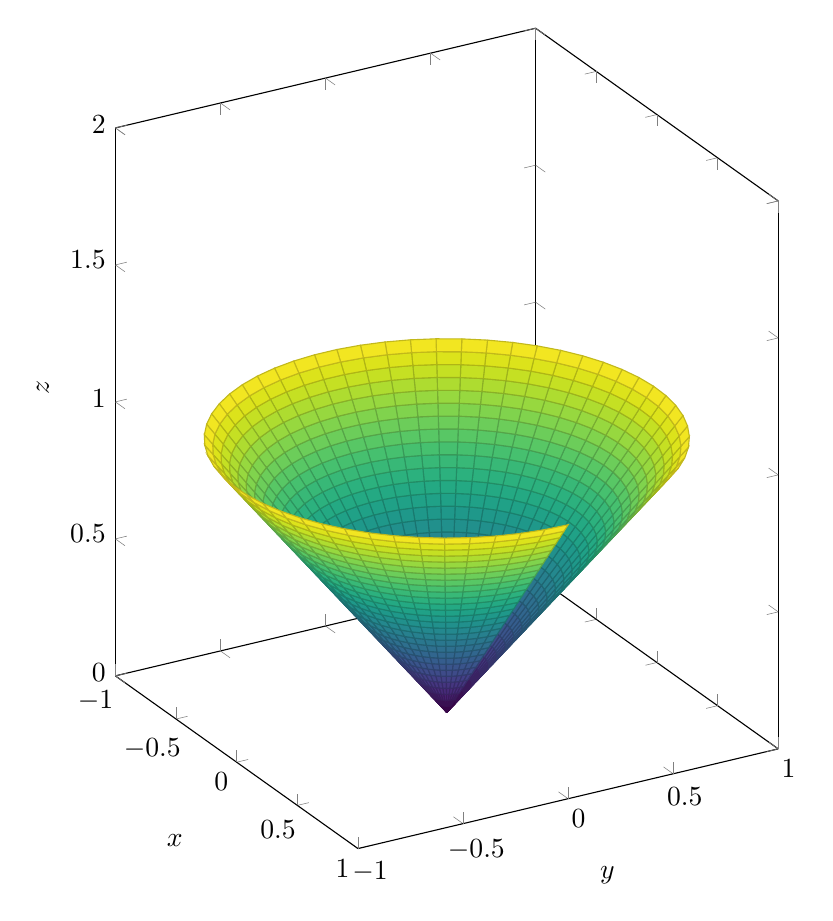
\begin{tikzpicture}
            \begin{axis}[
                    view={60}{20},
                    xlabel=$x$,
                    ylabel=$y$,
                    zlabel=$z$,
                    xmin=-1,
                    ymin=-1,
                    zmin=0,
                    xmax=1,
                    ymax=1,
                    zmax=2,
                    samples=50,
                    width=10cm,
                    height=12cm,
                    colormap/viridis,
                ]
                \addplot3[
            surf,
            domain=0:1,
            y domain=0:360,
            samples=30,
            samples y=60
        ]
        ({x*cos(y)},{x*sin(y)},{x}); % Parámetrico: x = r cos(θ), y = r sin(θ), z = r
            \end{axis}
        \end{tikzpicture}
    \end{center}

  

    La idea, es analizar la posibilidad de utilizar el teorema de Gauss. Podemos ver que $S$ no es una superficie cerrada.   Para ello, consideremos una superficie $S'$  cerrada tal  que $S \subseteq S'.$  Definamos   $S'=S\;\cup\;S_{tapa}\;$,  donde $S_1$, es la ``tapa'' superior que le "falta" al cono ``cortado''.  Algebraicamente $S_{tapa}=\{(x,y,z)\in \Re^{3} : x^2+y^2\le 1\;\land z=1\}$.

    Denotemos por $\Omega$  al cuerpo encerrado por $S'$. Al orientar $S'$ de manera exterior estamos en condiciones de usar el teorema de Gauss.
   \[
        \oiint _{S'} \mathbf{F}\cdot d\mathbf{A} =
        \iint _{S} \mathbf{F}\cdot d\mathbf{A} +
        \iint _{S_{tapa}} \mathbf{F}\cdot d\mathbf{A} +
        =\iiint _\Omega \grad \cdot \mathbf{F}\;dV \newline
     \]
    \[ 
        \iff \iint _{S} \mathbf{F}\cdot d\mathbf{A} =
        \iiint _\Omega \grad \cdot \mathbf{F}\;dV -
        \iint _{S_{tapa}} \mathbf{F}\cdot d\mathbf{A} 
    \]
   

    Resolvemos el primer t\'ermino.
    \begin{align*}
        \iiint _\Omega \grad \cdot \mathbf{F}\;dV = \iiint _\Omega3\:dV = 3\:\text{Vol}(\Omega)
    \end{align*}
    Pasando a  $\Omega$ en coordenadas cil\'indricas
    \[\begin{dcases}
            x=\rho \cos \phi \\
            y=\rho \sen \phi \\
            z=z
        \end{dcases}\] donde, $$0\leq\rho\leq z\:\land\:0\leq\phi\leq 2\pi \land 0\leq z \leq 1.$$

    Entonces nos queda    \[
        \text{Vol}(\Omega) =  \int_0^1  \int_0^{2\pi} \int_0^z  \rho\:d\rho\:d\phi \:dz=2\pi  \int_0^1\Big( \frac{\rho^2}{2}\Big|_0^z \Big) \:dz =  \pi   \int_0^1   z^2  \:dz= \frac{ \pi}{3}.
    \] Por lo cuál, 
     \begin{align*}
        \iiint _\Omega \grad \cdot \mathbf{F}\;dV =\pi
    \end{align*}

    Para clacular el segundo término, debemos parametrizar $S_{tapa}$.  Sea  $D_{\text{tapa}} = \{ (\rho, \phi) \in \mathbb{R}^2 : 0 \leq \rho \leq 1, \, 0 \leq \phi < 2\pi \}$ y  sea  $$\boldsymbol{\Sigma}:D_{tapa}\subset\Re^2\to\Re^3  \mbox{ tal que }   \boldsymbol{\Sigma}(\rho,\phi)=(\rho\cos(\phi),\rho\sin(\phi),1).$$
    Entonces podemos reescribir
    \[
        \iint _{S_{tapa}} \mathbf{F}\cdot d\mathbf{A}=\iint _{D_{tapa}} (\mathbf{F}\circ\boldsymbol{\Sigma})\cdot
        (\boldsymbol{\Sigma}_{\rho}\times\boldsymbol{\Sigma}_{\phi})\:d\mathbf{A}.
    \]
    Primero calculamos las derivadas parciales de la parametrizaci\'on.
    \begin{align*}
        \boldsymbol{\Sigma}_{\rho} & =(\cos(\phi),\sin(\phi),0) \\
        \boldsymbol{\Sigma}_{\phi} & =(-\rho \sin(\phi),\rho \cos(\phi),0)
    \end{align*}
    Entonces
    \[
        \boldsymbol{\Sigma}_{\rho}\times\boldsymbol{\Sigma}_{\phi}=(0,0,r)=\boldsymbol{\eta}.
    \]
    Podemos observar que $\boldsymbol{\eta}$ preserva la orientaci\'on  para $S_{tapa}$ heredada  por la orientaci\'on exterior de $S'$ elegida anteriormente para poder aplicar el teorema de Gauss, ya que $r\geq0$. En otras palabras,  $\boldsymbol{\eta}$ ``apunta''  hacia el exterior de $\Omega$.  
   
    Calculamos el término, 
    \[
         \iint _{D_{tapa}} (\mathbf{F}\circ\boldsymbol{\Sigma})\cdot
        (\boldsymbol{\Sigma}_{\rho}\times\boldsymbol{\Sigma}_{\phi})\:d\mathbf{A}=\int_0^1  \int_0^{2\pi}   \rho\:d\rho\:d\phi =2\pi  \Big( \frac{\rho^2}{2}\Big|_0^1 \Big) \:dz =  \pi   
    \]

    $$\therefore\;\iint _{S} \mathbf{F}\cdot d\mathbf{A}=\pi - \pi=0$$
\end{solution}

%------------Solucion 2---------------------------------------

\begin{solution}
En primer lugar, vamos a encontrar los puntos $P$ donde la superficie $S$ intersecta la curva $C$. Escribiremos las ecuaciones que definen a la curva $C $ en terminos de $y$:
   \[
   \begin{cases}
   y^2 - 2y - z + 1 = 0 \\
   y - x = 1
   \end{cases}
   \iff
   \begin{cases}
    z= y^2 - 2y  + 1 \\
    x =y- 1
   \end{cases}
  \]
Sustituyendo estos valores de y en las ecuaciones paramétricas de la curva, obtenemos los puntos de intersección
 \[
    (y^2 - 2y + 1) + (y - 1)^2 + (y - 1)^2 = 3
 \]
Expandiendo los términos y factorizando llegamos a que
 \[
    3y(y - 2) = 0 \iff 
    \begin{cases}
    y=0\\
    y=2
    \end{cases}
 \]

Ahora simplemente reemplazamos en las ecuaciones de la curva para obtener los valores de $x$ y $z$, con lo cual determinamos dos puntos:
\[
    P_1=(-1,0,1)
 \]
\[
    P_2=(1,2,1)
 \]
\end{solution}
Ahora que obtuvimos los puntos, vamos a buscar cada plano tangente a la superificie $S$ en los puntos $P_1 $ y $ P_2$. Recordamos la formula de plano tangente a una superficie: $\pi: \grad f(xo,yo,zo).(x-xo,y-yo,z-zo)=0$, donde definimos $f$ como $f(x,y,z)=z + (y - 1)^2 + x^2-3$ y calculamos su gradiente
\[
   \grad f(xo,yo,zo)=(2x,2(y-1),1)\quad\backslash 
   \begin{cases}
   \grad f(-1,0,1)=(-2,-2,1)\\
   \grad f(1,2,1)=(2,2,1)
   \end{cases}
 \]
 Por último, calculamos los planos tangentes en cada punto
 \[
 \pi_1: (-2,-2,1)(x+1,y,z-1)=0 \iff -2x-2-2y+z-1=0\iff -2x-2y+z-3=0
 \]
 \[
 \pi_2: (2,2,1)(x-1,y-2,z-1)=0 \iff 2x-2+2y-4+z-1=0\iff 2x+2y+z-7=0
 \]
\newline
$\therefore\;$ Los planos tangentes a $S$ en $P$ para cada punto $P \in (S \cap C)$ son:
\[
\pi_1:-2x-2y+z=3\quad \text {para  }  P_1=(-1,0,1)
 \]
 \[
 \pi_2:2x+2y+z=7\quad \text {para  }  P_2=(1,2,1)
 \]


%------------Solucion 3---------------------------------------

\begin{solution}
    Empezamos gráficando la curva a analizar, la cual se recorre en sentido antihorario
   \begin{center}
    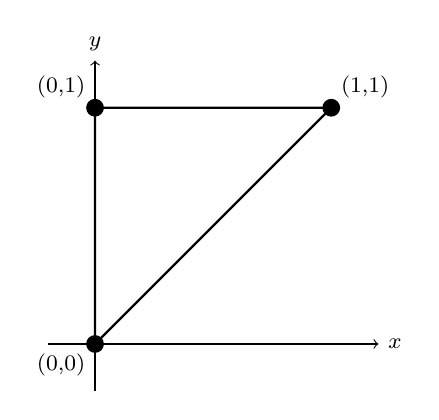
\begin{tikzpicture}[scale=3]
        % Ejes coordenados
        \draw[->] (-0.2,0) -- (1.2,0) node[right] {\footnotesize $x$};
        \draw[->] (0,-0.2) -- (0,1.2) node[above] {\footnotesize $y$};

        % Puntos
        \filldraw (0,0) circle (1pt) node[below left] {\footnotesize (0,0)};
        \filldraw (1,1) circle (1pt) node[above right] {\footnotesize (1,1)};
        \filldraw (0,1) circle (1pt) node[above left] {\footnotesize (0,1)};
        
        % Lados del triángulo
        \draw[thick] (0,0) -- (1,1) -- (0,1) -- cycle;
    \end{tikzpicture}
\end{center}
    Se nos solicita calcular la circulación del campo vectorial $F$ a lo largo de la curva cerrada $C$, siendo $F(x,y)=(xy,\sqrt{y^2+1)}$
    \[
\oint_C xy \, dx + \sqrt{y^2+1} \, dy = \oint_C(xy,\sqrt{y^2+1)}dxdy
\]
Como hablamos de una curva cerrada, simple y orientada en sentido antihorario, utilizamos el teorema de Green. En el mismo, la región $D$ encerrada la definimos como $D = \{ (x, y) \in \mathbb{R}^2 : 0 \leq y \leq 1, \, 0 \leq x < y \}$ la cuál graficamos para comprenderla mejor:
  \begin{center}
        \begin{tikzpicture}
            \begin{axis}[
                    axis lines=center,
                    axis equal,
                    xlabel=$x$,
                    ylabel=$y$,
                    xmin=0,
                    xmax=1,
                    ymin=0,
                    ymax=1.2,
                    xtick distance=1,
                    ytick distance=1,
                ]
                \addplot[name path=A, draw=none]{x} node[pos=0.55, right]{$y=x$};
                \addplot[name path=B, draw=none]{1};
                \addplot[fill=violet!90, opacity=0.7]fill between[of=A and B, soft clip={domain=0:1}];
            \end{axis}
        \end{tikzpicture}
    \end{center}

Por lo tanto, tenemos que 
\[
 \oint_C(xy,\sqrt{y^2+1)}dxdy=\iint _D \mathbf{rot(F)}\cdot d\mathbf{A}=\iint _D 0-x\cdot d\mathbf{A}=-\iint _D x\cdot d\mathbf{A}
\]
Utilizando los extremos de integración de la region $D$, resolvemos
 \[
         -\iint _D x\cdot d\mathbf{A}=-\int_0^1  \int_0^{y}   x\:dx\:dy =-  \int_0^1\Big( \frac{x^2}{2}\Big|_0^y \Big) \:dy=-\Big( \frac{y^3}{6}\Big|_0^1 \Big)=-\frac{1}{6}
    \]
$$\therefore\;\oint_C xy \, dx + \sqrt{y^2+1} \, dy =-\frac{1}{6}$$


\end{solution}

%------------Solucion 4---------------------------------------

\begin{solution}
 En primer lugar, podemos identificar que $\Omega $  es una elipsoide, por lo cuál vamos a comenzar realizando una transformación de la misma a coordenadas esfericas

\[
T(x,y,z) = \left( \frac{1}{4} \rho \cos(\theta)\sin( \varphi), \frac{1}{2} \rho \sin(\theta)\sin( \varphi),  \rho \cos(\varphi) \right)
\]
Donde $\Omega^*$ es el dominio transformado en coordenadas esféricas, definido por
 \[\Omega^*=\begin{cases}
            \;\rho \in [0,1] \\[5pt]
            \; \varphi \in [0,\pi] \\[5pt]
            \;\theta \in [0,2\pi]
        \end{cases}
    \]
De esta manera $T:\Omega^* \rightarrow \Omega$ es una transformación, cuyo determinante de la matriz Jacobiana se puede calcular utilizando el conocido de esfericas y la ayuda de la nota:

\[
J_T(\rho, \theta,\varphi) = \left| \det D_T (\rho, \theta,\varphi) \right| = \frac{1}{4}\frac{1}{2}\rho^2\sin(\varphi)
\]
Para empezar a demostrar la igualdad, partiremos del término izquierdo, donde definiremos una función $g:\Re^3\rightarrow\Re, g(x,y,z)=f(\sqrt{16x^2 + 4y^2 + z^2})$

\[
\iiint_\Omega f(\sqrt{16x^2 + 4y^2 + z^2}) \, dV=\iiint_{\Omega^*}g \circ T (\rho, \theta,\varphi).J_T(\rho, \theta,\varphi)dV=\iiint_{\Omega^*}f(\rho) \frac{1}{8}\rho^2\sin(\varphi)dV
\]
Resolviendo la integral,
\[
\frac{1}{8}\iiint_{\Omega^*}f(\rho) \rho^2\sin(\varphi)dV=\frac{1}{8}\int_0^{1} f(\rho) \rho^2d\rho.\int_0^{2\pi}d\theta.\int_0^{\pi}\sin(\varphi)d\varphi= \frac{\pi}{2}\int_0^{1} f(\rho) \rho^2d\rho
\]

$$\therefore\;\iiint_\Omega f(\sqrt{16x^2 + 4y^2 + z^2}) \, dV = \frac{\pi}{2}\int_0^{1} f(\rho) \rho^2d\rho$$

\end{solution}
